\chapter{The \linkDD* step}
\label{chap:2dlink}

The \link* step aims to link together consecutive time instants, by joining the coordinates of each individual bubble across the varius time instants it is seen.
The result is a series of \textbf{tracklets}.
Specifically, the 2D version of the \link* step operates on 2D coordinates, producing 2D tracklets.

\section{Requirements}

\subsection{Input}

The input to the \link* step coincides with the output of the previous step.
In the pipeline is using \linkDD*, the full pipeline under exam is \locate* - \link* - \match* - \visual*.
This means that the input to this step is the output of the \locate* step, as described in section~\ref{sec:locate:output}.

\subsection{Output}
\label{sec:linkDD:output}

The coordinates of the particles in the tracklets follow the same format as the \locate* output.
A four-dimensional \texttt{positions} array describes the \texttt{(x, y)} coordinates of the bubbles inside \texttt{positions[C][F][B]}, $C$, $F$ and $B$ being the camera, frame and bubble indices, respectively.
The difference with the \locate* format is that values of $B$ are scoped across the whole acquisition, not limited to the single frame.
This means that all values with the same $C$ and $B$ will represent the same real bubble across the different frames.

With this representation, valid bubbles are not clusterized at the smallest values of $B$: for example, bubble $B{=}0$ may disappear after some frames, leaving the rest of its tracklet to contain invalid positions.
As such, the \texttt{numTracers} array is not anymore enough to describe the valid positions.
Instead, a different array is used: \texttt{validTracers} is a three-dimensional, boolean array.
\texttt{validTracers[C][F][B]} contains the information of whether the bubble $B$ of camera $C$ was detected at frame $F$.
False values indicate that, at a specific frame, the bubble was either not found yet, or already lost, or the overall number of bubbles traced by camera $C$ was lower than $B$.

\subsection{Speed}

As for the \locate* step, each second the \linkDD* has to process the bubbles from $N{\cdot}f$ frames, where $N$ is the number of cameras and $f$ is their framerate.
As such, the required speed for this step is the same 90 FPS that is required by the \locate* step.

\subsection{Quality}

The overall quality of an algorithm can be estimated by combining manual observation with the number of resulting tracklets found.
For the manual observation, the input video was overlayed with a tail composed of points and segments, describing the last few frames of trajectory.
Figures~TODO are examples of frames used for manual observation: the single links are quite small, it is hard to see them individually, it's much easier to consider the general view.

Possible situations of reconstructed links are:
\begin{itemize}
	\itemsep 0em
	\item Link correctly detected: the number of total tracklets does not change from the previous frame, and the link is coherent with the rest of the trajectory;
	\item Link not detected: visually, it's hard to notice the missing link; however, this splits the tracklet into two pieces, increasing the number of tracklets by 1;
	\item Wrong link detected: the number of tracklets remains the same, while an inconsistent movement is visible by eye.
\end{itemize}
As such, a good reconstrucion is one with few tracklets and a coherent visual representation.

\section{State of the art}

For the \link* step, online research was less successful: no new approach was found, and only some of the libraries found for the \locate* step were also performing the task:
\begin{itemize}
	\itemsep 0em
	\item Section~\ref{sec:link2d:trackpy} explores the Trackpy~\cite{trackpy} Python library;
	\item Section~\ref{sec:link2d:myptv} explores the MyPTV~\cite{myptv} Python library.
\end{itemize}
As for the \link* step, they are described and evaluated in the following chapters.

\section{Approaches}

The following sections describe the different approaches evaluated for the \linkDD* step.
They are evaluated on a 201-frames video~\cite{linkDD-original}, whose frames look like figure~\ref{fig:locate:original}.
For the different approaches, a crop of a sample frame is reported as per the \locate* approaches (section~\ref{sec:locate:approaches}), with the tail of the tracklet.
Full videos are available on YouTube, following the links in the corresponding citations.

\newpage
\subsection{Trackpy}
\label{sec:link2d:trackpy}

The \texttt{link} function from the Trackpy~\cite{trackpy} library is able to perform the \link* task both in 2D and in 3D.

Originally, it required the located positions to be inside a \texttt{Pandas Dataframe}, and it used to convert it into a \texttt{NumPy} array.
However, since our data was already inside a \texttt{NumPy} array with the same format, the library was altered to avoid this useless conversion, thus saving time.

\subsubsection{Algorithm}

The Trackpy library implements the Crocker-Grier linking algorithm~\cite{trackpy-link}.

\subsubsection{Evaluation}

For a single camera, the linking speed was 40 FPS.
If different cameras were analyzed in parallel processes, 3 cameras could be processed at an overall speed of 120 FPS.

The quality was good at a visual inspection (see figure~\ref{fig:linkDD:trackpy} or the full video~\cite{linkDD-trackpy}), and the total number of tracklets was around 6500.

\begin{figure}
	\centerline{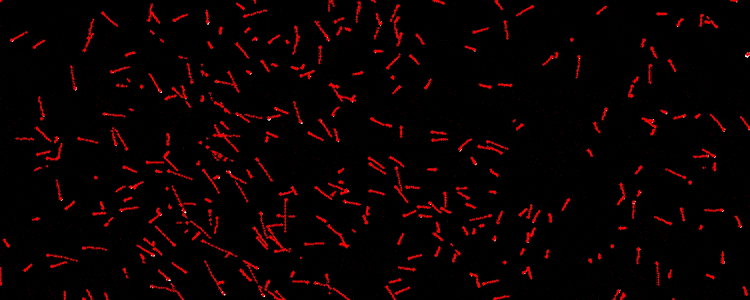
\includegraphics[width=\locateimgsize]{images/link2d/trackpy.png}}
	\caption{\centering A frame from the Trackpy \linkDD* result, full video available at~\cite{linkDD-trackpy}}
	\label{fig:linkDD:trackpy}
\end{figure}
 \newpage
\subsection{MyPTV}
\label{sec:link2d:myptv}

...

\subsubsection{Algorithm}

...

\subsubsection{Evaluation}

...

% \begin{figure}
% 	\centerline{\includegraphics[width=\locateimgsize]{images/link/...}}
% 	\caption{\centering ...'s result}
% 	\label{fig:locate:...}
% \end{figure}
 \newpage
\subsection{Kalman CPU}
\label{sec:link2d:kalman-cpu}

...

\subsubsection{Algorithm}

...

\subsubsection{Evaluation}

...

% \begin{figure}
% 	\centerline{\includegraphics[width=\locateimgsize]{images/link/...}}
% 	\caption{\centering ...'s result}
% 	\label{fig:locate:...}
% \end{figure}
 \newpage
\subsection{Kalman GPU}
\label{sec:link2d:kalman-gpu}

The Kalman CPU approach performs the same operation over all the bubbles of all the images.
A GPU implementation was therefore evaluated, to test its potential parallelization.

\subsubsection{Algorithm}

The algorithm is the same as the previous approach, with step 2 transformed into a GPU kernel.
This kernel processes all bubbles of all images captured at the same time instant.

\subsubsection{Evaluation}

The speed is quite faster than the Kalman CPU approach, but still considerably slower than Trackpy, standing at 68 FPS.
The quality was however worse: the number of tracklets increased to about 8900, and a visual inspection found some inconsistencies (in figure~\ref{fig:linkDD:kalmangpu}, two trackelts include an unreasonable jump).

\begin{figure}
	\centerline{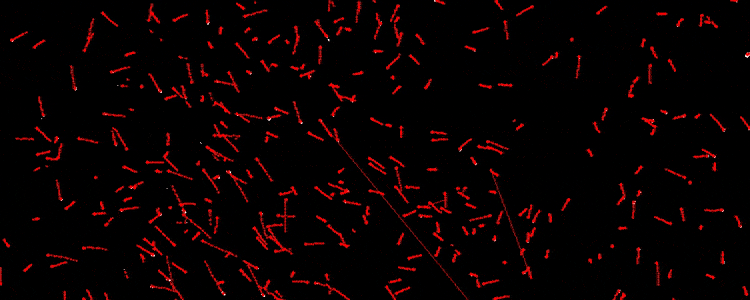
\includegraphics[width=\locateimgsize]{images/link2d/kalman_GPU.png}}
	\caption{\centering A frame from the Kalman GPU \linkDD* result, full video available at~\cite{linkDD-kalman-gpu}}
	\label{fig:linkDD:kalmangpu}
\end{figure}
 \newpage

\section{Final choice}

Figure~\ref{fig:linkDD:speed} compares the speeds of the various \linkDD* approaches: Trackpy is the only one with an adequate speed.
On top of that, it is also the approach with the best overall quality.
As such, if the pipeline is traversed in the \locate* - \link* - \match* - \visual* order, the \link* step will use the Trackpy implementation.

\begin{figure}
	\centerline{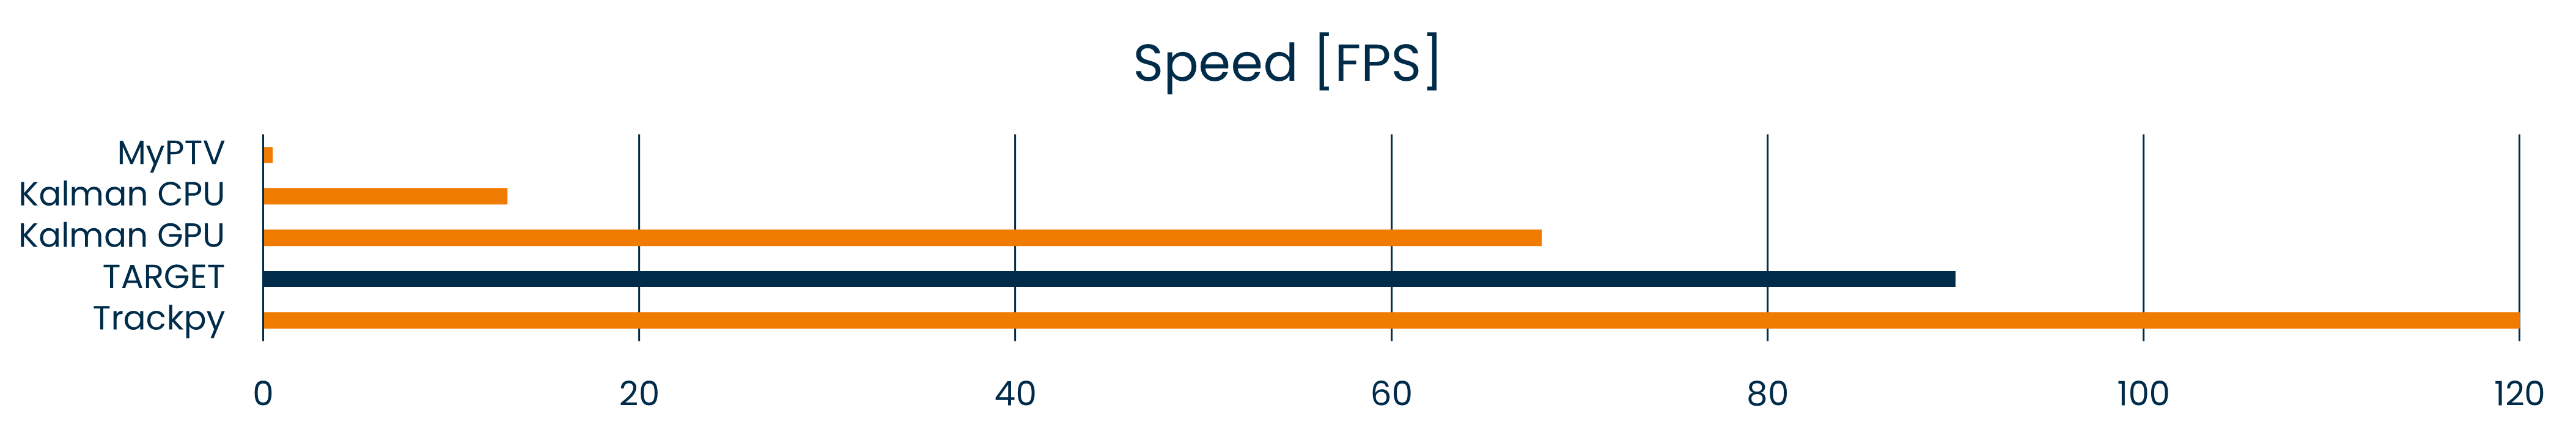
\includegraphics[width=\locateimgsize]{images/link2d-speed-comparison.png}}
	\caption{\centering Comparing the speeds of the different \linkDD* approaches}
	\label{fig:linkDD:speed}
\end{figure}
